\section{Opstelling}
Het belangrijkste element voor een immersieve opstelling is een head-mounted
display. Traditioneel zijn HMDs met grote field of view zeer duur en niet 
beschikbaar voor consumenten, maar tegenwoordig zijn er enkele betaalbare HMDs 
beschikbaar met een redelijk grote field of view, zoals de Oculus Rift DK1 
(110\textdegree{} diagonaal), zie Figuur \ref{fig:or-dk1}.

\begin{figure}[b!]
    \centering
    \includegraphics[width=0.7\textwidth, angle=90]{or-dk1}
    \caption{De Oculus Rift Developer Kit 1, met de retroreflectieve bolletjes
    voor het tracking systeem.}
    \label{fig:or-dk1}
\end{figure}

Om een vloeiende werking te verzekeren werd de virtuele omgeving gedraaid op een
Apple MacBook Pro met een 2,5 GHz Intel Core i5 processor, 8 GB 1333 MHz DDR3 RAM
geheugen en een Intel HD Graphics 4000 GPU. Het beeld werd getoond op een Oculus 
Rift (Devkit 1) aan 60 fps voor beide ogen. Deze HMD heeft een diagonale FoV van 
110\textdegree{} en vult hierdoor bijna het hele zicht van de proefpersonen voor 
een maximale immersie.

Het is voor immersie ook belangrijk dat de positie van de proefpersoon in de 
fysieke omgeving zeer precies geweten is. Tracking van positie en rotatie in 3 
assen werd gedaan door een 6 camera OptiTrack systeem rondom een 3 m x 4 m 
tracking gebied. Om gebruikersinvoer te voorzien werd er een bluetooth muis 
gebruikt, zodat de proefpersoon op een knop kon klikken om het object in beeld te
activeren. Een foto van deze volledige opstelling, met een proefpersoon die het
experiment is aan het ondernemen is te zien in Figuur \ref{fig:tester}


\section{Beschrijving}
Elke testpersoon kreeg een briefing waar hem verteld werd dat hij door een 
virtueel kantoor zou gaan wandelen. Ik deelde hem mee dat hij in elk kantoor de 
blinden zou moeten sluiten met de knop naast het raam, en dat hij de foto boven 
deze knop moest onthouden. Vervolgens werd hem gevraagd het kantoor te verlaten 
en de deur achter hem te sluiten en dit proces voor 3 kantoren te herhalen. Er
werd verder verteld dat interactie met het object in beeld gebeurt door op de
muisknop te klikken.

Vervolgens werd er gevraagd of er onduidelijkheden waren en begaven we ons naar 
de startpositie, de proefpersoon werd de Oculus Rift aangeboden om zelf op te 
zetten en aan te passen aan zijn hoofd. Na de uitvoering van het experiment werd 
de proefpersoon een korte vragenlijst voorgelegd om in te vullen.

\begin{figure}[t!]
    \centering
    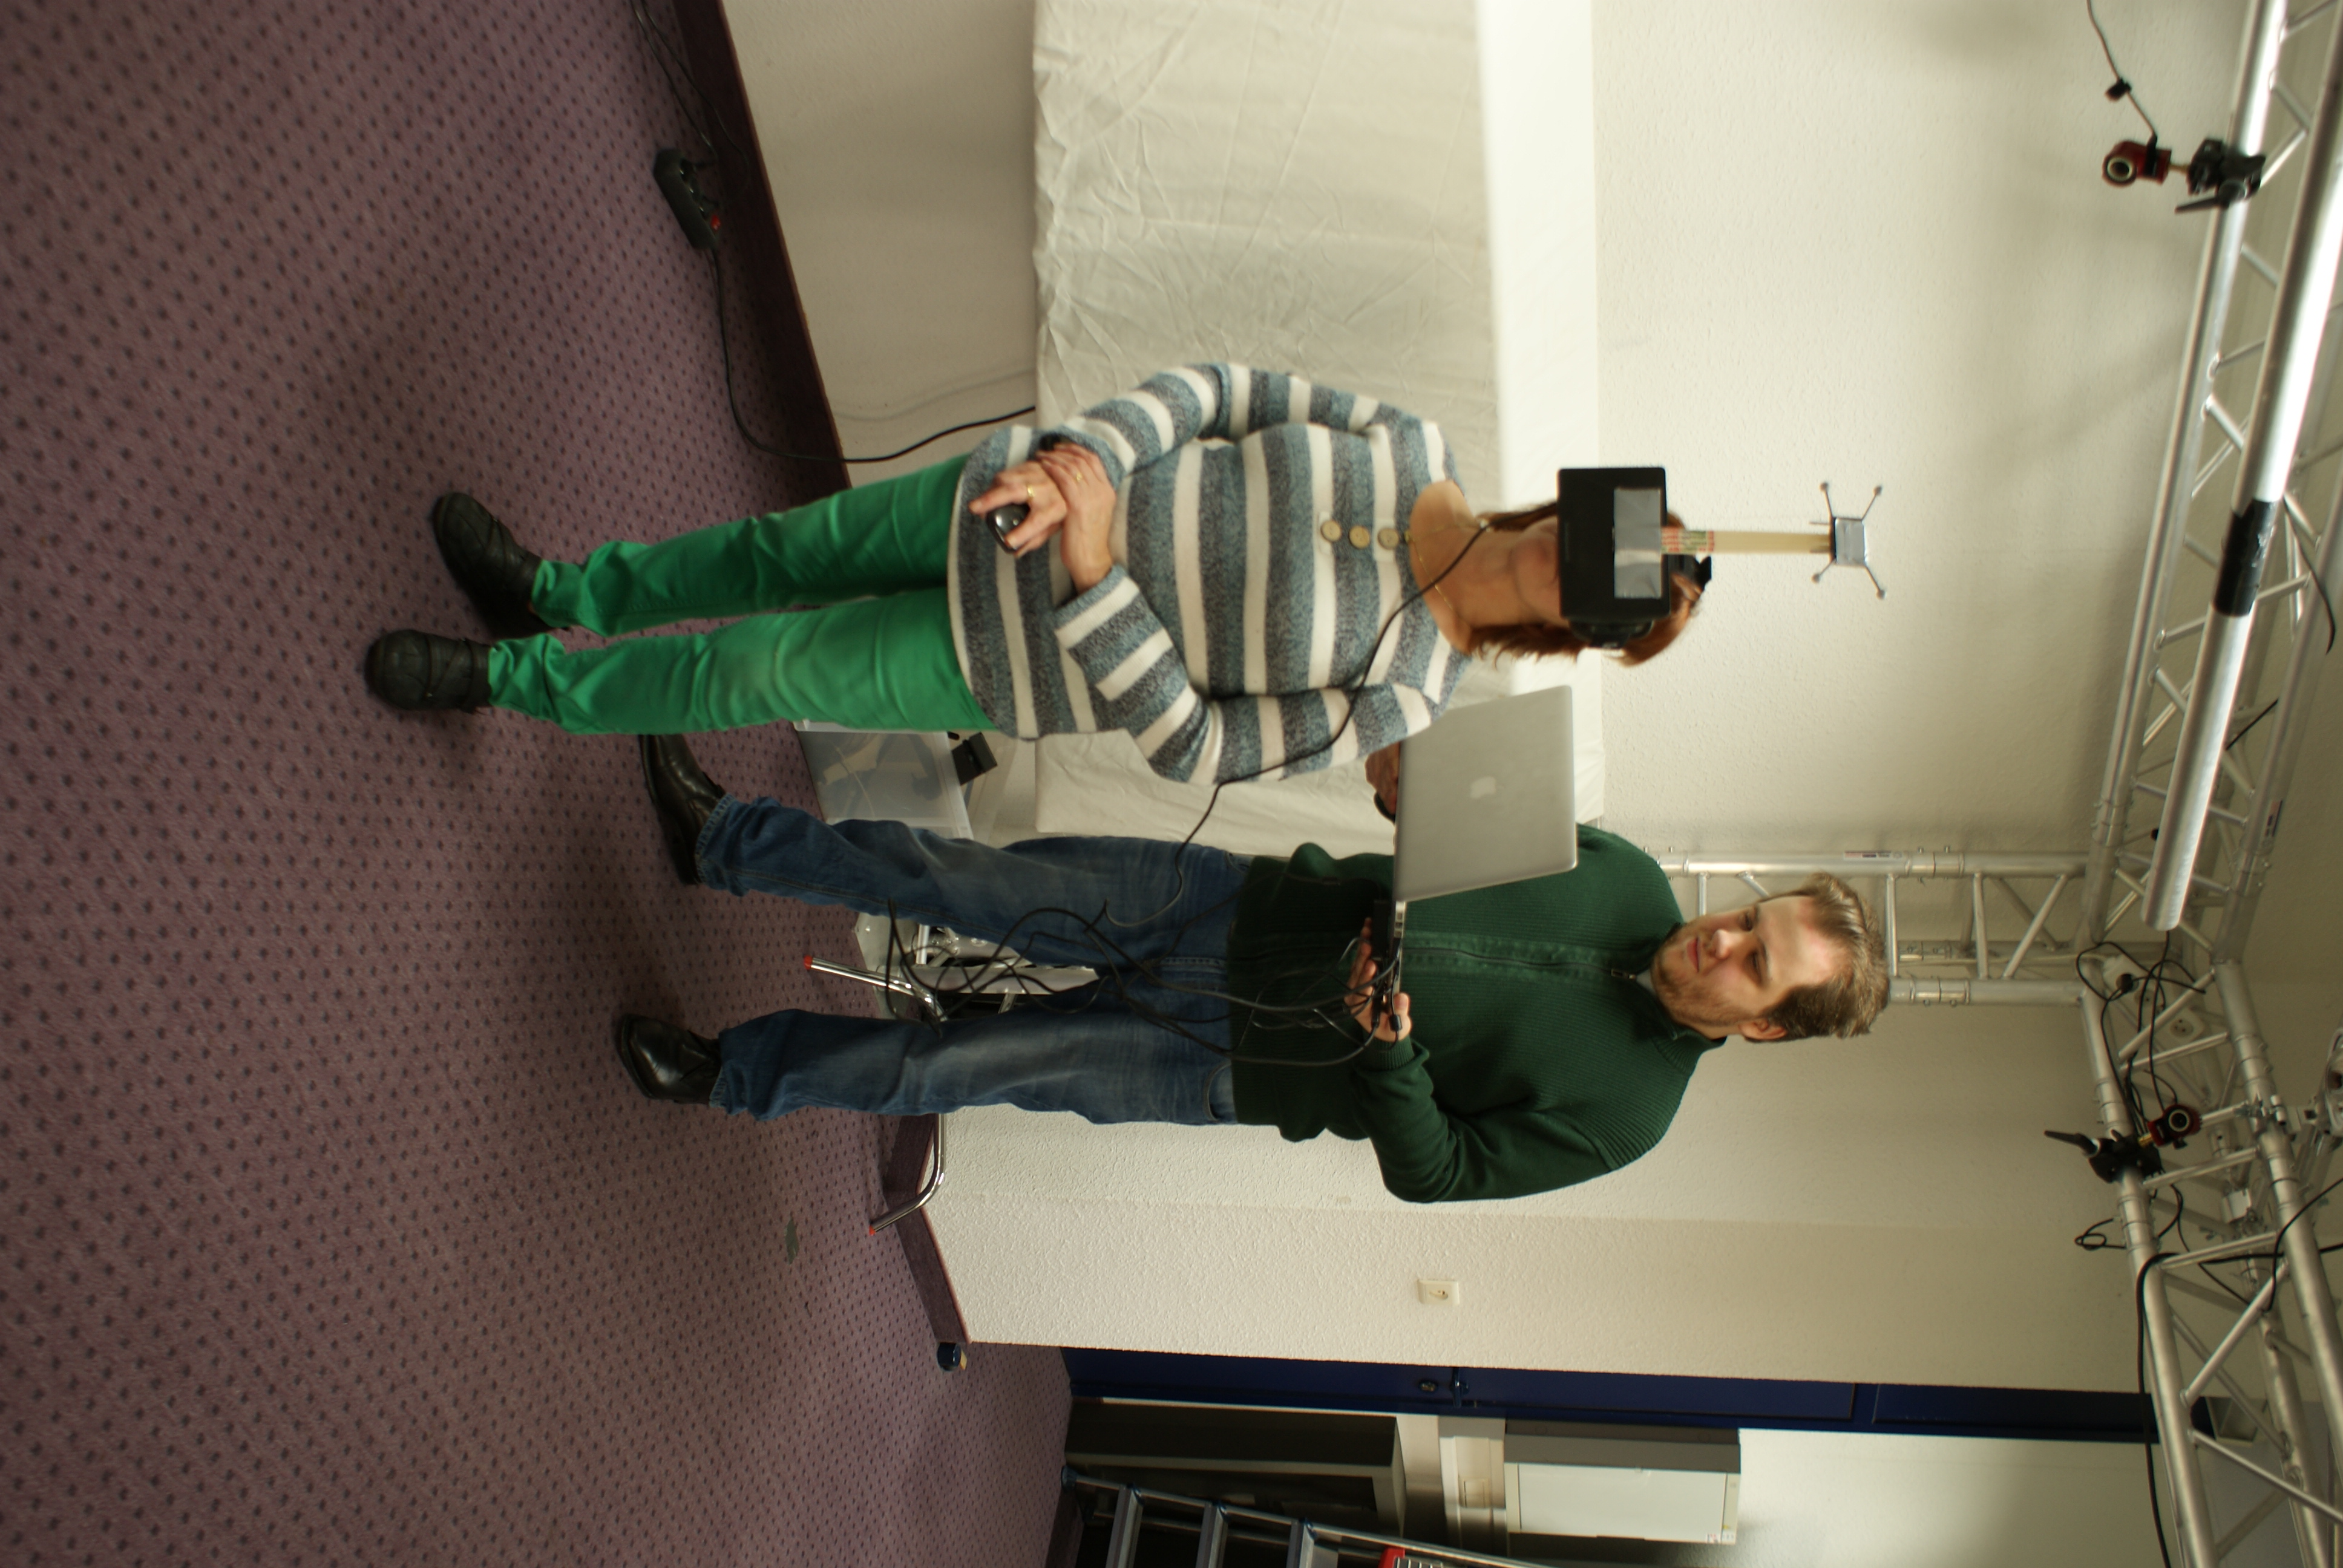
\includegraphics[width=0.7\textwidth, angle=90]{testsubject}
    \caption{Een proefpersoon met de Oculus Rift op, terwijl ze door de virtuele
    omgeving is aan het wandelen. Merk ook de tracking camera's op die aan het
    kader hangen.}
    \label{fig:tester}
\end{figure}


\section{Vragenlijst}
De vragenlijst bestaat uit een gebied voor algemene informatie en vijf specifieke
vragen. Deze vragenlijst werd wegens de diversiteit van de proefpersonen in het
Nederlands en het Engels beschikbaar gesteld. De Nederlandse versie van de 
vragenlijst is ingevoegd in Bijlage \ref{vragenlijst}. Als algemene informatie 
wordt er gevraagd naar de leeftijd, het geslacht en de voorkennis van de 
proefpersoon, dit om te analyseren of er verschillen in effectiviteit tussen 
deze groepen zijn. 

Vervolgens wordt er gevraagd om een schema van het grondplan te tekenen, om te
zien of er ondanks de onmogelijke ruimte toch een consistent mentaal beeld kon
gevormd worden. Daarna wordt er gevraagd om de drie fotos op te noemen. Deze
vraag is niet verwerkt in de resultaten daar deze een onderdeel uitmaakt van de
afleiders. In vraag drie moet de proefpersoon aan acht stellingen een score 
toekennen van 1 tot 6 waar 1 betekent dat hij het niet heeft gemerkt, en 6 dat 
het heel duidelijk wel is gebeurd:

\begin{enumerate}
  \item Ik zag de virtuele omgeving groter of kleiner worden.
  \item \emph{Ik voelde alsof ik het zelfde pad aan het belopen was.}
  \item Ik zag de virtuele omgeving flitsen.
  \item \emph{Ik merkte dat iets in de omgeving zich van plaats had veranderd.}
  \item Ik zag de virtuele omgeving roteren.
  \item Ik voelde mezelf groter of kleiner worden.
  \item Ik voelde me alsof ik bewogen werd.
  \item Ik merkte dat iets in de virtuele omgeving groter of kleiner werd.
\end{enumerate}

Enkel de schuingedrukte stellingen zijn echt gebeurd, de andere stellingen zouden
een zeer lage gemiddelde score moeten hebben. De laatste twee vragen bestaan uit 
een vraag waar wordt gevraagd voor algemene qualitatieve feedback over de 
immersie, en een vraag waar wordt gevraagd om de bewogen voorwerpen te 
identificeren.

De vragenlijst is gebaseerd op de vragenlijst uit het eerdere experiment van Evan
A. Suma\cite{suma11} om onze resultaten met die van dat onderzoek te kunnen 
vergelijken.


\section{Implementatie}
\subsection{Engine}
Voor de implementatie van de virtuele omgeving heb ik er voor gekozen om met de
Unity engine te werken. Ik heb deze keuze gemaakt omdat de Unity engine relatief
eenvoudig is om mee te werken en mij meer tijd over laat om te werken aan de
benodigde algoritmen. Voor het ontwerp van de omgeving heb ik gebruik gemaakt 
van de Blender 3D editor, wegens eerdere ervaring met deze editor. Ik beschrijf 
nu even kort mijn implementatie.


\subsubsection{Interactie}
Bij de activatie van deuren en knoppen wordt er eerst gekeken of de proefpersoon
zich op minder dan een meter afstand van het object bevind, en of hij het object
in beeld heeft. Als aan beide voorwaarden wordt voldaan wordt de animatie
geactiveerd. Unity heeft ingebouwde functionaliteit om een punt via een
matrixtransformatie te transformeren van wereldco\"ordinaten naar 
viewportco\"ordinaten.


\subsubsection{Animatie}
Voor de animaties maak ik gebruik van sferische lineaire interpolatie tussen de
begin- en de eindpositie van de te animeren objecten. Ook deze functionaliteit
wordt door Unity voorzien.

Voor de \emph{animatie} van de beweging van de gang wordt deze gewoon in een keer
verplaatst, omdat deze niet in het zicht van de proefpersoon is. Daar de deuren 
in het object van de gang verwerkt zitten, is deze beweging de effectieve
implementatie van change blindness in de virtuele omgeving zoals beschreven in
Paragraaf \ref{1:blindness}.


\subsection{Tracking}
Voor integratie met het trackingsysteem heb ik gebruik gemaakt van de gratis
editie van de MiddleVR middleware\cite{middlevr}. Deze maakt het mogelijk om via 
het VRPN protocol te communiceren met de tracking server.

MiddleVR geeft ook toegang tot \emph{virtual trackers} waarmee men de data van 
een tracker kan transformeren. Het resultaat hiervan is dat ik de pitch en de 
roll van de HMD heb kunnen gebruiken, en de yaw van het camera tracking systeem. 
Dit omdat de HMD een kleine hoeveelheid \emph{yaw drift} heeft, en dit zou kunnen 
zorgen voor botsingen met de fysieke omgeving. Een schema van de manier waarop ik
de verschillende inputs gebruik is te zien in Figuur \ref{fig:sensorfusion}. Het
ook op dit punt dat de positie in het XY-vlak met 1.1 wordt vermenigvuldigd om
een effectieve snelheid van 110\% te bekomen.

\begin{figure}[t!]
    \centering
    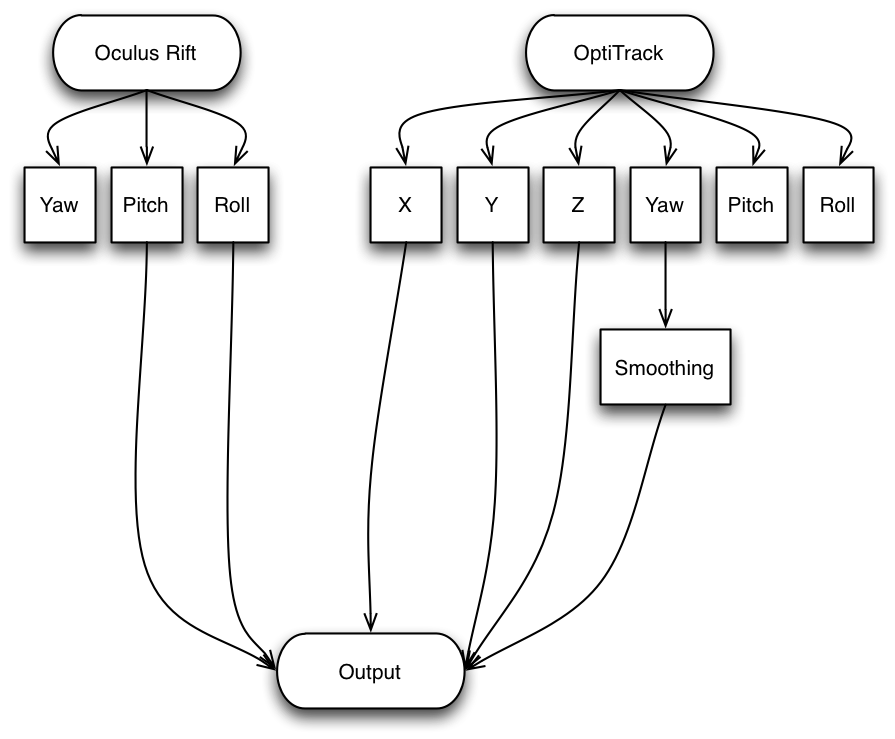
\includegraphics[width=0.7\textwidth]{sensorfusion}
    \caption{Schema van de samengevoegde sensor inputs.}
    \label{fig:sensorfusion}
\end{figure}

Aan de serverkant heb ik gebruik gemaakt van de standaard OptiTrack:Motive 
software om de VRPN data te broadcasten.
